\documentclass[thesis.tex]{subfiles}

\begin{document}

    \section{Analysis of Wafer 292}
    \label{sec:wafer292}

        Of wafer 292, the membranes 292c and 292d have been measured. The pores were opened by floating as explained in \cref{sssec:barrier-layer-dissolution}. The thickness of the membranes is
        \begin{equation}
            l_\mathrm{pore}=\SI{60}{\micro\meter}.
        \end{equation}
        Expected is an absorption and desorption isotherm with a hysteresis as explained in \cref{sssec:open-funnelled-pores}.


    \section{Analysis of Wafer 296}
    \label{sec:wafer296}

        The thickness of wafer 296 is
        \begin{equation}
            l^{296}_\mathrm{pore}=SI{60}{\micro\meter}.
        \end{equation}
        As explained before in \cref{sssec:barrier-layer-dissolution}, this wafer shall be used to further understand the barrier layer dissolution. The goal is to be able to produce the membranes in a more controlled way an to hereby reduce the funneling aspect of the pores. \cref{fig:wafer-296} shows the treatments of the membranes and gives an overview over the conducted measurements. While the membranes 296c and 296d are immersed in ??? acid for
        \begin{align}
            \begin{split}
                t^\mathrm{296c}_\mathrm{immerse}=\SI{6,5}{\minute},    \\
                t^\mathrm{296d}_\mathrm{immerse}=\SI{13}{\minute},
            \end{split}
            \label{eq:t-immerse}
        \end{align}
        296e and 296f are only floated on the acid on the barrier layer side for
        \begin{align}
            \begin{split}
                t^\mathrm{296e}_\mathrm{float}=\SI{13}{\minute}, \\
                t^\mathrm{296f}_\mathrm{float}=\SI{26}{\minute}
            \end{split}
            \label{eq:t-float}
        \end{align}
        respectively. Assuming the etch rate to be equal for both sides of the barrier layer, meaning from within the pore and from the outside, the thickness of the barrier layer of 296c and 296e and also of 296d and 296f should be equal after the dissolution. Moreover, all pores should still be closed assuming an etch rate of approximately $\SI{1}{\nano\meter\per\minute}$. The latter should be clearly visible on the volumetric measurements. Furthermore, only the pores of the immersed membranes are expected to be widened. The horizontal etch rate which, according to \cref{sssec:barrier-layer-dissolution} must be different from the one attacking the barrier layer vertically, shall be put a figure to in the run of the evaluations.

        \subfile{tikz/wafers/wafer_296_processing_plan.tex}

        \Cref{fig:full-comp-w296} shows a full comparison of the volumetric measurements of the membranes mentioned above. Additionally, membrane 296a is drawn on the graph. Its barrier layer remains untouched making for closed pores. The comparison of the different membranes implies that indeed, all pores are still closed as the shapes of the isotherms of the four treated membranes match the one of 295a and no big diameter variation can be observed. Which cannot be observed though, that is weather the pores already have microscopic openings on the barrier layer side. If that were the case, hexane would condense there at spinodal pressures lower than the equilibrium pressure of the small ends. Hereby, the pores would be left in a closed shape. This case would not be visible on the volumetric measurements as the condensed amount of hexane necessary to close the pores were so small. If the openings were so large already as for the spinodal pressure to be larger than the equilibrium pressure of the small end, that case would be visible on the isotherm because whole pores would fill at higher pressures. Therefore, the latter case can be excluded.
        ???REFER TO THE THEORY PORE THEORY SECTION HERE ???

        Next, the floated and immersed membranes shall be regarded separately.

        \begin{figure}[ht]
            \centering
            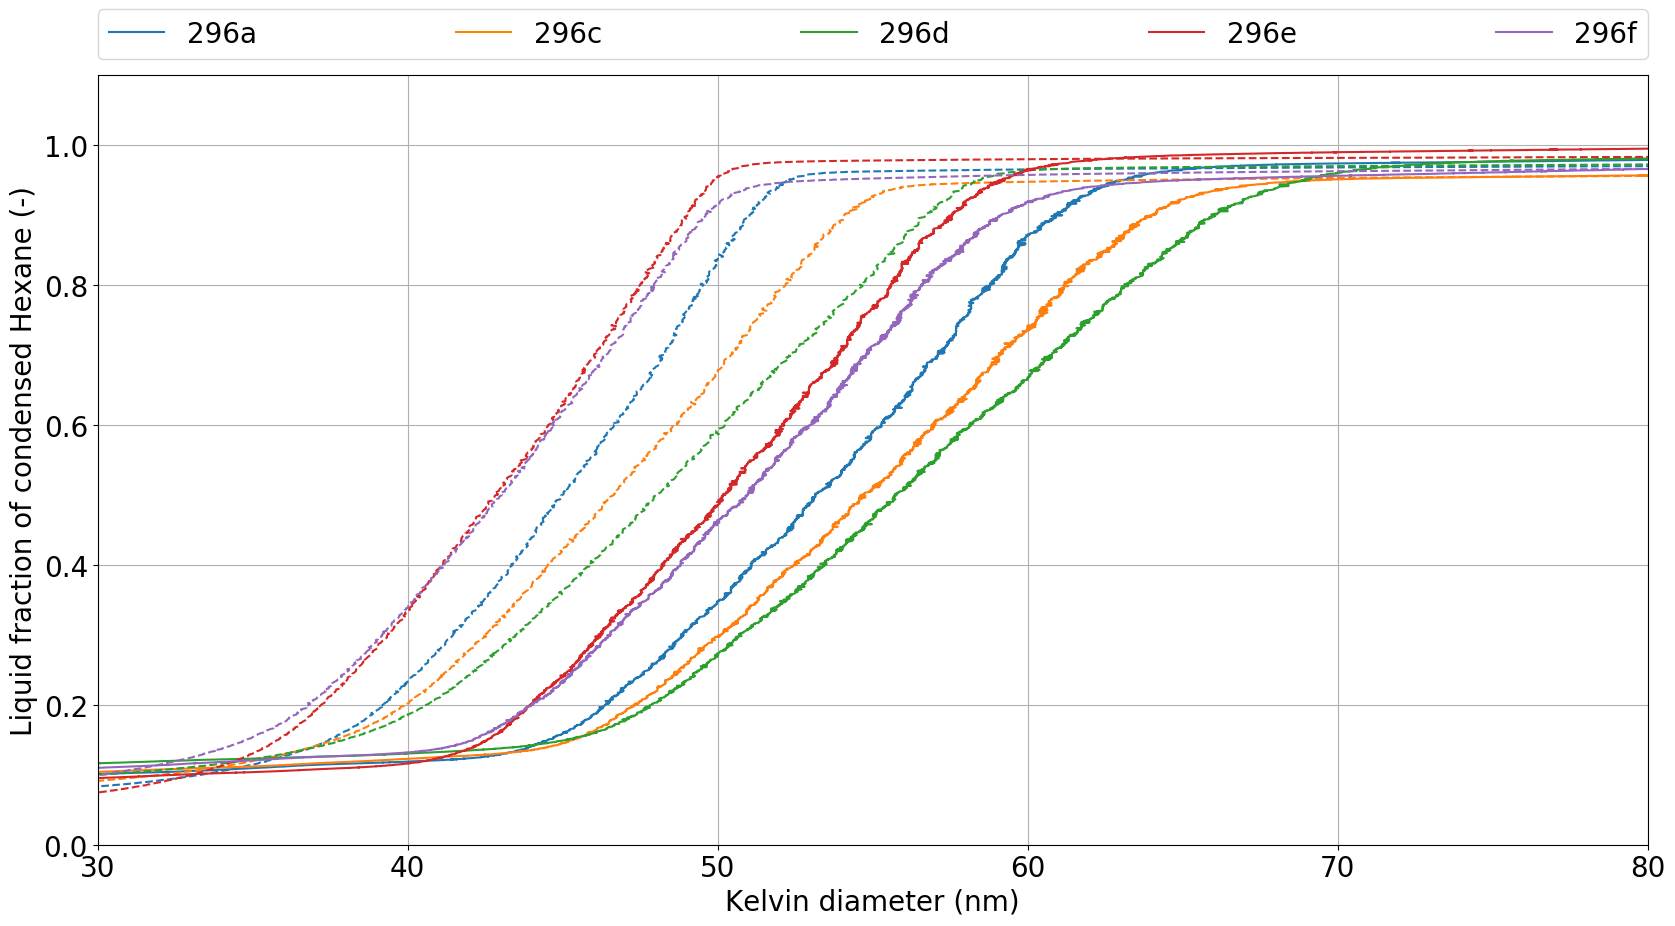
\includegraphics[width=\textwidth]{images/296a_vs_296c_vs_296d_vs_296e_vs_296f_d_kelvin.png}
            \caption{Comparison of the volumetrically measured membranes of wafer 296 on a \textsc{Kelvin} diameter axis. The solid lines represent the condensation whereas the dashed lines correspond to the evaporation of an isotherm cycle. As 296a is a membrane with closed pores (untouched barrier layer), by comparison it is clearly visible that the rest of the membranes, as expected, have closed pores too.}
            \label{fig:full-comp-w296}
        \end{figure}


        \subsection{Floated Membranes 296e and 296f}
        \label{subsec:floated-membranes}

            \begin{figure}[ht]
                \centering
                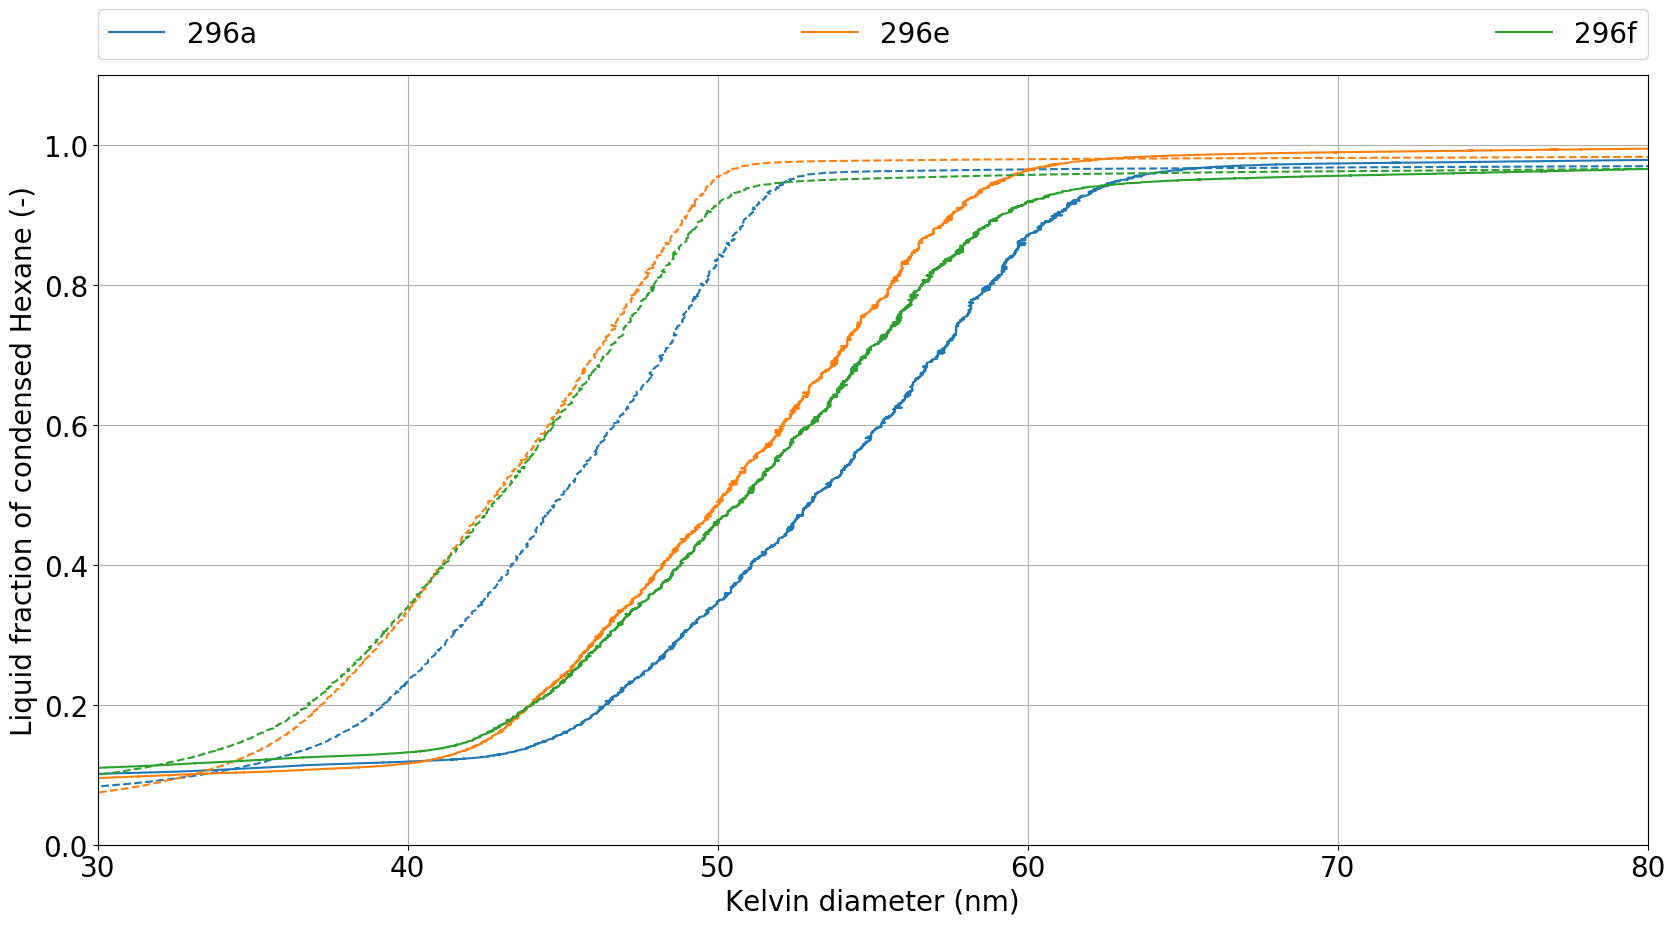
\includegraphics[width=\textwidth]{images/296a_vs_296e_vs_296f_d_kelvin.png}
                \caption{Comparison of 296a, 296e and 296f on a \textsc{Kelvin} diameter axis. }
                \label{fig:floated-comp-w296}
            \end{figure}

            ??? OPTICAL ANALYSIS STILL MISSING ???

            The comparison of the volumetric measurements of the three membranes is shown in \cref{fig:floated-comp-w296}. Even though the wafer has been produced as a whole and the membranes 296e and 296f have only been floated on ??? acid without opening the pores, by theory leaving the pore diameters unchanged, a clear offset in diameter between 296a and the other two membranes is visible. As 296e and 296f are pretty superimposed though and also the shapes of isotherms match according to \cref{sec:wafer296}, no error in the before made interpretations of the pores still being closed can be implied. This leaves only the possibility of the pore diameters being distributed throughout the wafer and hereby throughout the membranes.


        \subsection{Immersed Membranes 296c and 296d}
        \label{subsec:immersed-membranes}

            \subfile{tikz/graphs/immersion_experiment/immersion.tex}

            \Cref{fig:immersed-comp-w296} compares the volumetric measurements of the immersed membranes 296c and 296d, again adding the untreated membrane 296a. As explained in \cref{sssec:cfp-leo}, condensation and evaporation in a closed funnelled pore occur at equilibrium pressure. Pores that are open on the large end start filling from the bottom and evaporating from the top so, regarding the isotherms in \cref{fig:immersed-comp-w296}, the lower end of the isotherm rising represents the small bottom end of the pores. This lower end of all three isotherms seems to be superimposed while the top end, representing the large open end of the pores, moves to larger diameters for longer immersion times. As the effect seems to occur linearly over the whole length of the pores, the acid seems to be saturating within the pores losing etching power. By \cref{sssec:cfp-leo}, the process can be visually interpreted as shown in ???. Moreover, the increase of the funnelling aspect seems to be linear at least within the first 13 minutes of the immersion as doubling the immersion time yields double the diameter shift on the volumetric isotherm (compare \cref{eq:t-immerse}).

            \subfile{tikz/wafer_analysis/funnelling_increase.tex}


    \section{Analysis of Wafer 295}
    \label{sec:wafer295}

        Wafer 295 is only
        \begin{equation}
            l^{295}_\mathrm{pore}=\SI{30}{\micro\meter}
        \end{equation}
        thick. Hereby, the funneling observed upon the previously measured membranes of a thickness of
        \begin{equation}
            l^{292,293,294,296}_\mathrm{pore}=\SI{60}{\micro\meter}
        \end{equation}
        is supposed to be reduced. Assuming that the funneling aspect is linear implies a reduction of the effect by half. \Cref{fig:wafer_295} shows the treatments and measurements of the inspected membranes of wafer 295.

        \subfile{tikz/wafers/wafer_295_processing_plan.tex}

        \subsection{Membrane 295a}

            To start with, membrane 295a shall be analysed. It is untreated, meaning that the pores are still closed on one end by the barrier layer. Expected are straight pores of a diameter of approximately
            $\SI{40}{\nano\meter}$ diameter with a significantly reduced funneling aspect resulting in a rather upright evaporation isotherm. The result is displayed in ???. The absorption and desorption isotherm shows a king at two thirds of the height, which cannot easily be explained. While for straight pores, a straight isotherm rising is expected, the observed kink could speak for a deformation as shown in ???, assuming that it is due to intra pore defects, not inter pore defects. Regarding inter pore defects, a discreet pore diameter variation could cause this shape of isotherm. Again, the reason for such a discreet distribution in pore sizes is not clear.


            \subsubsection{Membrane 295a - after Aluminum Dissolution Bath}

                Membrane 295a is measured again after a bath in the ??? acid. The point of this is to see, if the  wafers immersion in the acid when dissolution the remaining aluminum after the anodizing might cause any unexpected defects or pore widening already. As the anodizing of wafer 295 has been conducted with the same parameters as the other wafers before (for instance wafer 296, the pore diameters are expected to be approximately the same. Referring to wafer 296 the pore diameters of
                \begin{equation*}
                    d_\mathrm{pore}^\mathrm{296a} = \SI{45\pm 5}{\nano\meter}
                \end{equation*}
                do not fit the ones results of membrane 295a with
                \begin{equation*}
                    d_\mathrm{pore}^\mathrm{295a} = \SI{55\pm 6}{\nano \meter}.
                \end{equation*}
                Finally, the probing of the aluminum dissolution process, which by theory is not supposed to attack the alumina of the membranes and therefore has not been taken a deeper look at, yields the before and after result displayed in \cref{fig:295-al-before-after}. In between the two measurements, the membrane has been immersed for
                \begin{equation*}
                    t_\mathrm{immerse} = \SI{4,5}{\hour}
                \end{equation*}
                in ??? acid at a temperature of
                \begin{equation*}
                    T_\mathrm{acid} = \SI{0}{\celsius}.
                \end{equation*}
                The aluminum dissolution of the wafers takes approximately
                \begin{equation}
                    t_\mathrm{Al diss.} = \SI{4}{\hour}
                \end{equation}
                and uses the same parameters which makes for a relevant approximation of what changes to the pores are expected during the before mentioned production step. The change to the pore diameters is
                \begin{equation}
                    \Delta d_\mathrm{pore}^\mathrm{Al diss.} = \SI{3}{\nano\meter}.
                \end{equation}
                Both, the starting points of the condensation rise and of the evaporation drop are shifted in the same way. Moreover, the hysteresis did not increase during the process. These two observations speak for the pore widening being homogeneous and also the corrugations not having increased during the etching. Therefore, the production step of the aluminum dissolution conducted as explained in \cref{sssec:al-dissolution} can be disregarded as a cause of big pore impurities.

                \begin{figure}[ht]
                    \centering
                    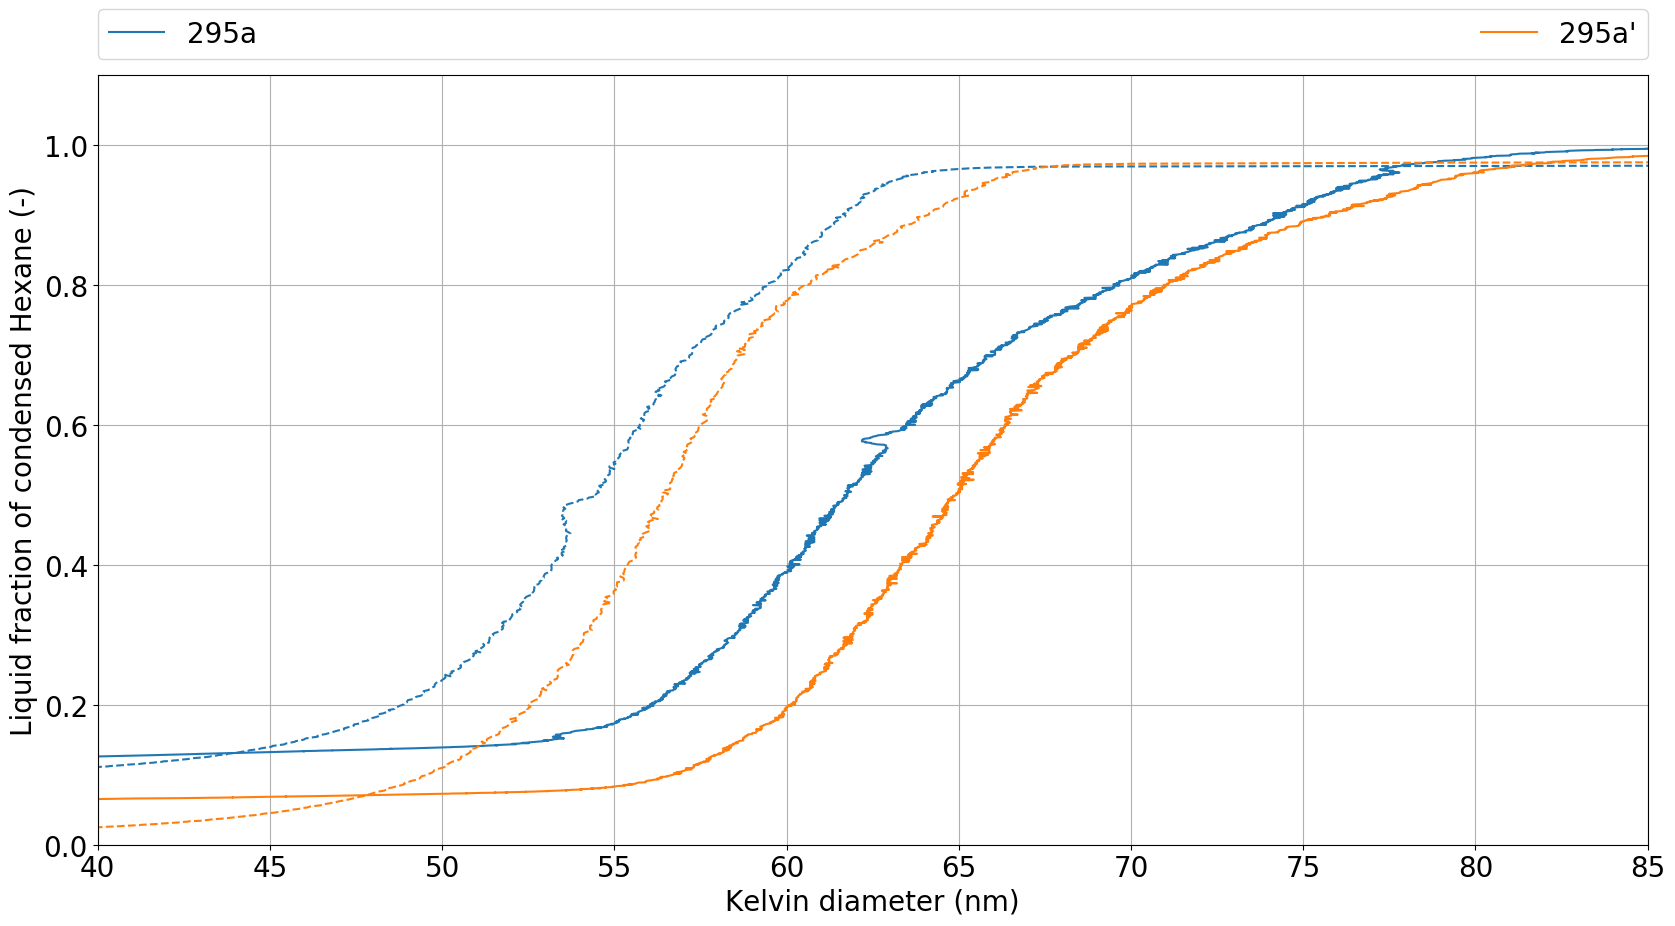
\includegraphics[width=\textwidth]{images/295a'_vs_295a_d_kelvin.png}
                    \caption{Comparison of the isotherms recorded for membrane 295a before and after the aluminum dissolution bath. Due to the homogeneous shift of the isotherm one can draw the conclusion that the aluminum dissolution process does not cause severe pore impurities.}
                    \label{fig:295-al-before-after}
                \end{figure}


        \subsection{Membrane 295d, 295e, 295f, 295g}

            The membranes 295d, 295e, 295f, 295g yield very upright isotherms without any kinks or transmission defects. On the contrary, the membranes 295e and 295f superimpose perfectly, while 295d and 295g are only shifted to larger diameters ???. For all the membranes, the transmission dips of absorption and desorption show the same value. This can only be explained by almost perfectly straight pores if the disorder theory in \cref{subsec:light-transmission-interpretation} are assumed to be correct. Also, regarding the conversion to pore diameters according to \textsc{Kelvin} equation (compare \cref{sec:kelvin-equation}, the funneling aspect is the weakest so far measured in this experiment. This can be explained by the inverse of the effect observed upon the opening experiments of wafer 296 ???.


        \subsection{Membrane 295c}


\end{document}
